%%%%%%%%%%%%%%%%%%%%%%%%%%%%%%%%%%%%%%%%%
% Beamer Presentation
% LaTeX Template
% Version 1.0 (10/11/12)
%
% This template has been downloaded from:
% http://www.LaTeXTemplates.com
%
% License:
% CC BY-NC-SA 3.0 (http://creativecommons.org/licenses/by-nc-sa/3.0/)
%
%%%%%%%%%%%%%%%%%%%%%%%%%%%%%%%%%%%%%%%%%

%----------------------------------------------------------------------------------------
%	PACKAGES AND THEMES
%----------------------------------------------------------------------------------------

\documentclass{beamer}

\mode<presentation> {

% The Beamer class comes with a number of default slide themes
% which change the colors and layouts of slides. Below this is a list
% of all the themes, uncomment each in turn to see what they look like.

%\usetheme{default}
%\usetheme{AnnArbor}
%\usetheme{Antibes}
%\usetheme{Bergen}
\usetheme{Berkeley}
%\usetheme{Berlin}
%\usetheme{Boadilla}
%\usetheme{CambridgeUS}
%\usetheme{Copenhagen}
%\usetheme{Darmstadt}
%\usetheme{Dresden}
%\usetheme{Frankfurt}
%\usetheme{Goettingen}
%\usetheme{Hannover}
%\usetheme{Ilmenau}
%\usetheme{JuanLesPins}
%\usetheme{Luebeck}
%usetheme{Madrid}
%\usetheme{Malmoe}
%\usetheme{Marburg}
%\usetheme{Montpellier}
%\usetheme{PaloAlto}
%\usetheme{Pittsburgh}
%\usetheme{Rochester}
%\usetheme{Singapore}
%\usetheme{Szeged}
%\usetheme{Warsaw}

% As well as themes, the Beamer class has a number of color themes
% for any slide theme. Uncomment each of these in turn to see how it
% changes the colors of your current slide theme.

%\usecolortheme{albatross}
%\usecolortheme{beaver}
%\usecolortheme{beetle}
%\usecolortheme{crane}
%\usecolortheme{dolphin}
%\usecolortheme{dove}
%\usecolortheme{fly}
%\usecolortheme{lily}
\usecolortheme{orchid}
%\usecolortheme{rose}
%\usecolortheme{seagull}
%\usecolortheme{seahorse}
%\usecolortheme{whale}
%\usecolortheme{wolverine}

%\setbeamertemplate{footline} % To remove the footer line in all slides uncomment this line
%\setbeamertemplate{footline}[page number] % To replace the footer line in all slides with a simple slide count uncomment this line

%\setbeamertemplate{navigation symbols}{} % To remove the navigation symbols from the bottom of all slides uncomment this line
}
\usepackage{graphics}
\usepackage{graphicx} % Allows including images
\usepackage{booktabs} % Allows the use of \toprule, \midrule and \bottomrule in tables
%\usepackage{bibentry}
\usepackage{algorithm}
\usepackage[noend]{algpseudocode}
\usepackage{subcaption}
\captionsetup{compatibility=false}

% from report:
\usepackage{amsmath, amsthm, amssymb, amsfonts}

\newcommand{\R}{\mathbb{R}}
\newcommand{\N}{\mathbb{N}}
\DeclareMathOperator*{\argmin}{arg\,min}
\DeclareMathOperator*{\argmax}{arg\,max}
\DeclareMathOperator*{\minimize}{minimize}
\DeclareMathOperator*{\Argmin}{\text{Argmin}}
\DeclareMathOperator*{\Argmax}{\text{Argmax}}
\DeclareMathOperator*{\Cost}{\text{Cost}}
	
\newcommand{\indep}{\perp \!\!\! \perp}

%----------------------------------------------------------------------------------------
%	TITLE PAGE
%----------------------------------------------------------------------------------------

\title[Generative Images]{\textit{Article analysis:} Neural Optimal Transport} % The short title appears at the bottom of every slide, the full title is only on the title page

\author{Paul Barbier and Bastien Le Chenadec} % Your name
\institute[MVA, Ponts] % Your institution as it will appear on the bottom of every slide, may be shorthand to save space

\date{March 28, 2024} % Date, can be changed to a custom date

\begin{document}

\begin{frame}
    \titlepage% Print the title page as the first slide
\end{frame}

\begin{frame}
    \frametitle{Overview} % Table of contents slide, comment this block out to remove it
    \tableofcontents % Throughout your presentation, if you choose to use \section{} and \subsection{} commands, these will automatically be printed on this slide as an overview of your presentation
\end{frame}

%----------------------------------------------------------------------------------------
%	PRESENTATION SLIDES
%----------------------------------------------------------------------------------------

\section{Introduction}
\begin{frame}{Introduction}

\end{frame}

\section{Optimal Transport}

\subsection{The Problem}
\begin{frame}{Optimal Transport Problem}
    \begin{itemize}
        \item $\mu$, $\nu$ probability distributions on ${\cal X}$, ${\cal Y}$.
        \item Cost function: $c:{\cal X}\times\mathcal{\cal Y}\to\R$.
        \item Problem: finding a \textbf{transport map} $T^*:\mathcal{X}\to \mathcal{Y}$ such that:
    \end{itemize}

    \begin{equation}
        T^* \in \Argmin_{T\#\mu=\nu} \int_{\mathcal{X}} c(x,T(x))d\mu(x)
    \end{equation}

    where $(T\#\mu)(A)=\mu(T^{-1}(A))$ is the pushforward measure.

    Hence, one can define:

    \begin{equation}
        \Cost(\mu,\nu) = \int_{\mathcal{X}} c(x,T^*(x))d\mu(x)
    \end{equation}

\end{frame}

\begin{frame}{Kantorovich formulation: a relaxed OT problem}
    \begin{itemize}
        \item Let $\Pi(\mu,\nu)$ the set of distributions on $\mathcal{X}\times\mathcal{Y}$ with marginals $\mu$ and $\nu$.
        \item Problem: find a \textbf{transport plan} $\pi^*\in \Pi(\mu,\nu)$ such that:
    \end{itemize}
    \begin{equation}
        \pi^* \in \Argmin_{\pi\in\Pi(\mu,\nu)} \int_{\mathcal{X}\times\mathcal{Y}} c(x,y)d\pi(x,y)
    \end{equation}
    and we can define:
    \begin{equation}
        \Cost(\mu,\nu) = \int_{\mathcal{X}\times\mathcal{Y}} c(x,y)d\pi^*(x,y)
    \end{equation}
\end{frame}

\subsection{Weak OT Duality}
\begin{frame}{Weak OT Duality}
    For weak OT cost $C$ and a sufficiently regular function $f$,

    \begin{equation}
        f^C(x) = \inf_{\rho\in \mathcal{P}(\mathcal{Y})} \left\{C(x,\rho)-\int_{\mathcal{Y}}f(y)d\rho(y)\right\}
    \end{equation}
    where $\mathcal{P}(\mathcal{Y})$ denotes the set of probability distributions on $\mathcal{Y}$.

    Then, the dual form of the weak OT problem writes:

    \begin{equation}
        f^*\in\Argmax_{f} \int_{\mathcal{X}} f^C(x)d\mu(x) + \int_{\mathcal{Y}} f(y)d\nu(y)
    \end{equation}
    and the cost can be defined as follows
    \begin{equation}
        \Cost(\mu,\nu) = \int_{\mathcal{X}} f^{*C}(x)d\mu(x) + \int_{\mathcal{Y}} f^*(y)d\nu(y)
    \end{equation}

\end{frame}

\section{NOT}

\subsection{Weak dual OT reformulation}
\begin{frame}{Weak dual OT reformulation}
    \begin{itemize}
        \item $\mathcal{X}\subset\R^n$, $\mathcal{Y}\subset\R^m$ and $\mathcal{Y}\subset\R^d$.
        \item Let $\rho\in \mathcal{P}(\mathcal{Z})$ with some basic assumptions.
    \end{itemize}
    Then, we have:
    \begin{equation}
        f^C(x)=\inf_t \left\{C(x, T\#\rho)-\int_{\mathcal{Z}}f(t(z))d\rho(z)\right\}
    \end{equation}
    which leads to the maximin problem:
    \begin{equation}
        \Cost(\mu,\nu) = \sup_{f} \inf_{T} \mathcal{L}(f,T)
    \end{equation}

    where
    $\mathcal{L}(f,T) = \int_{\mathcal{Y}}fd\nu + \int_{\mathcal{X}} \left( C(x, T(x,\cdot)\#\rho)-\int_{\mathcal{Z}}f(T(x,z))d\rho(z)\right)d\mu(x)$
\end{frame}

\begin{frame}{The trick: noise outsourcing}
    \begin{itemize}
        \item Here, they introduce $T:\mathcal{X}\times\mathcal{Z}\to\mathcal{Y}$.
        \item Trick known as \textbf{noise outsourcing}:
    \end{itemize}

    \begin{theorem}
        If $X$ and $Y$ are random variables in suitable spaces ${\cal X}$ and ${\cal Y}$, then there exists $\eta\sim {\cal U}([0,1])$ with $\eta \indep X$ and a function $h\: [0, 1]\times {\cal X} \longrightarrow {\cal Y}$ such that $(X, Y) = (X, h(\eta, X))$ almost surely.
    \end{theorem}
\end{frame}

\begin{frame}{Weak OT: A summary}
    \begin{figure}
        \centering
        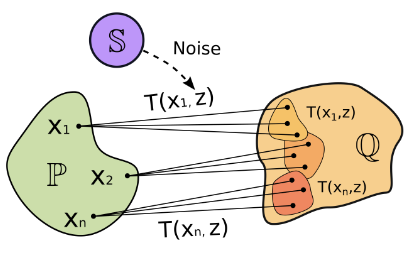
\includegraphics[width=0.9\linewidth]{figures/transportation-plan.png}
        \label{transportation-map}
        \caption{Transportation map with outsourced noise $z$ (taken from~\cite{korotin-2022})}
    \end{figure}
\end{frame}

\subsection{SGAD}
\begin{frame}{Stochastic Gradient Ascent Descent (SGAD)}
    TODO: Need to add the algorithm, couldn't do it easily with a rescalebox.
\end{frame}

\section{Experiments}

\subsection{Synthetic data}
\begin{frame}{Synthetic data}
    \begin{itemize}
        \item 2D standard normal distribution for $\mathcal{X}$.
        \item Moon distribution for $\mathcal{Y}$.
        \item Weak OT cost for $\gamma = 1$:
    \end{itemize}
    \begin{equation}
        C\big{(}x,\mu\big{)}=\int_{\mathcal{Y}}\frac{1}{2}\|x-y\|^{2}d\mu(y)-\frac{1}{2} \text{Var}(\mu)=\frac{1}{2}\|x-\int_{\mathcal{Y}}y\,d\mu(y)\|^{2}
        \label{eq:toy_cost}
    \end{equation}

    The parameters:
    \begin{itemize}
        \item simple feedforward model.
              \begin{itemize}
                  \item 2 hidden layers (100 units each).
                  \item ReLU activation.
              \end{itemize}
        \item Adam optimizer.
    \end{itemize}
\end{frame}

\begin{frame}{Results: the fitted distribution}
    \begin{figure}[H]
        \centering
        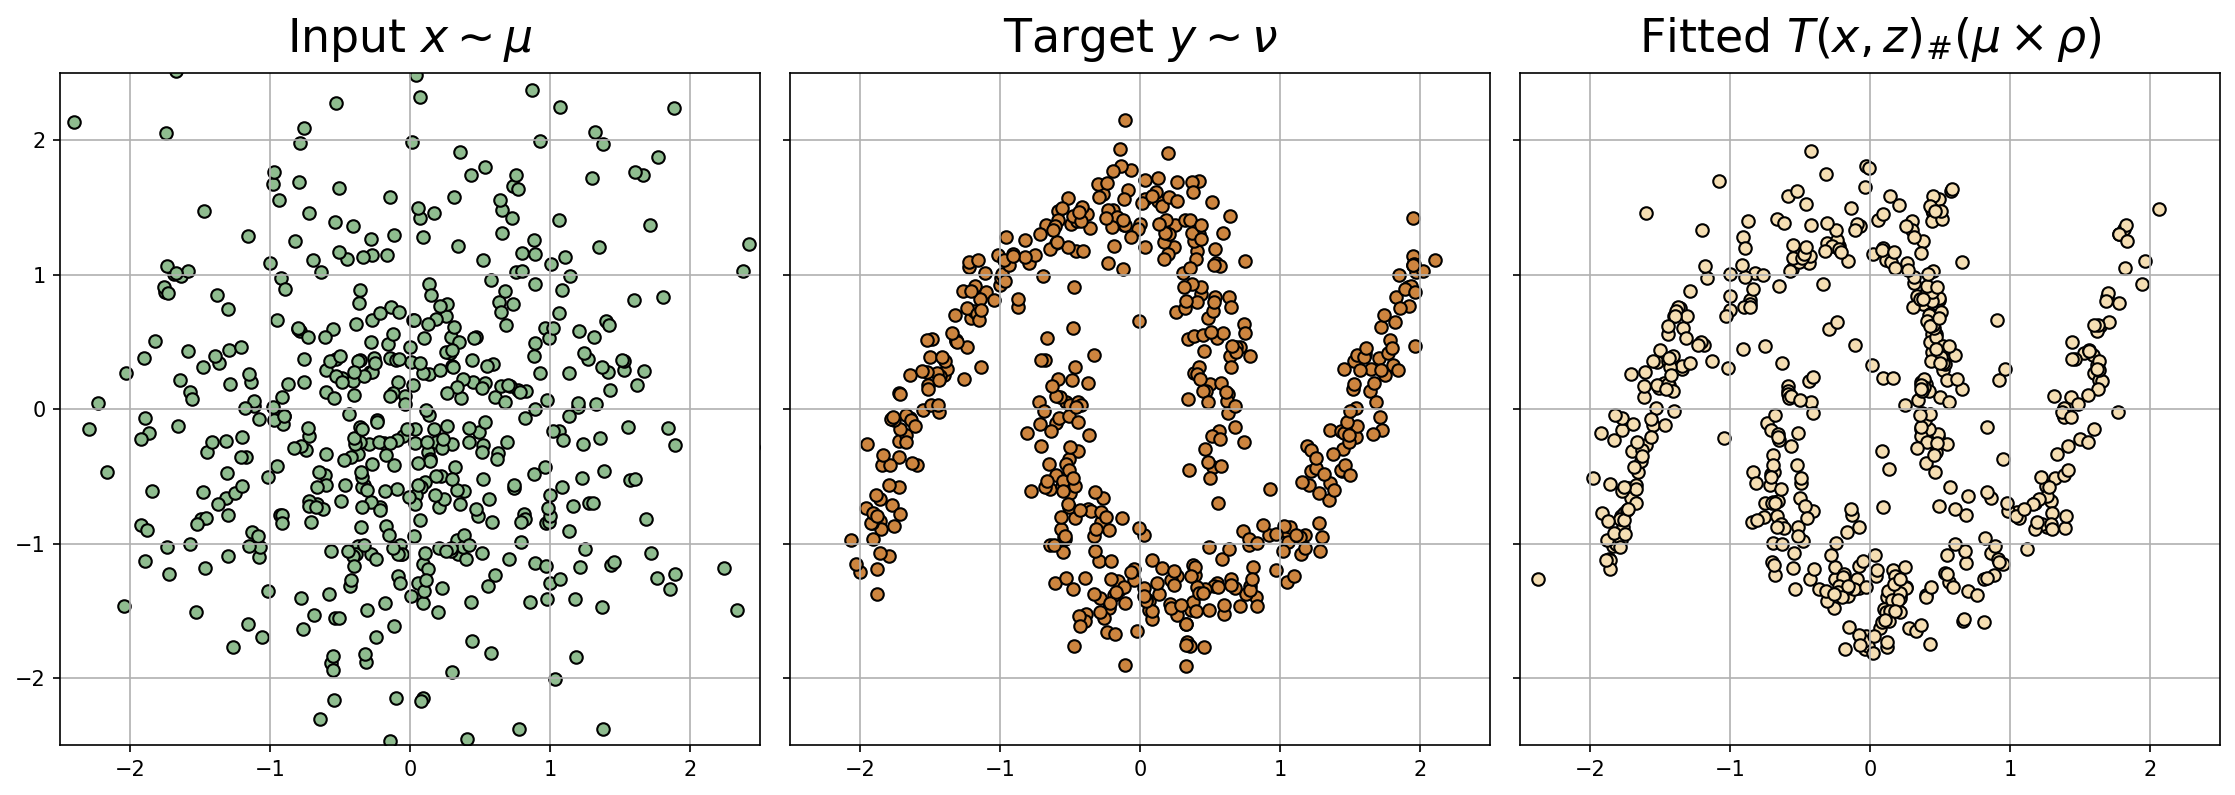
\includegraphics[width=0.9\textwidth]{figures/toy_1.png}
        \caption{Synthetic data experiment. Left: input gaussian distribution. Middle: target distribution. Right: learned transport of the input distribution to the target distribution.}
        \label{fig:toy_1}
    \end{figure}
\end{frame}

\begin{frame}{Results: a closer look at the map}
    \begin{figure}[H]
        \centering
        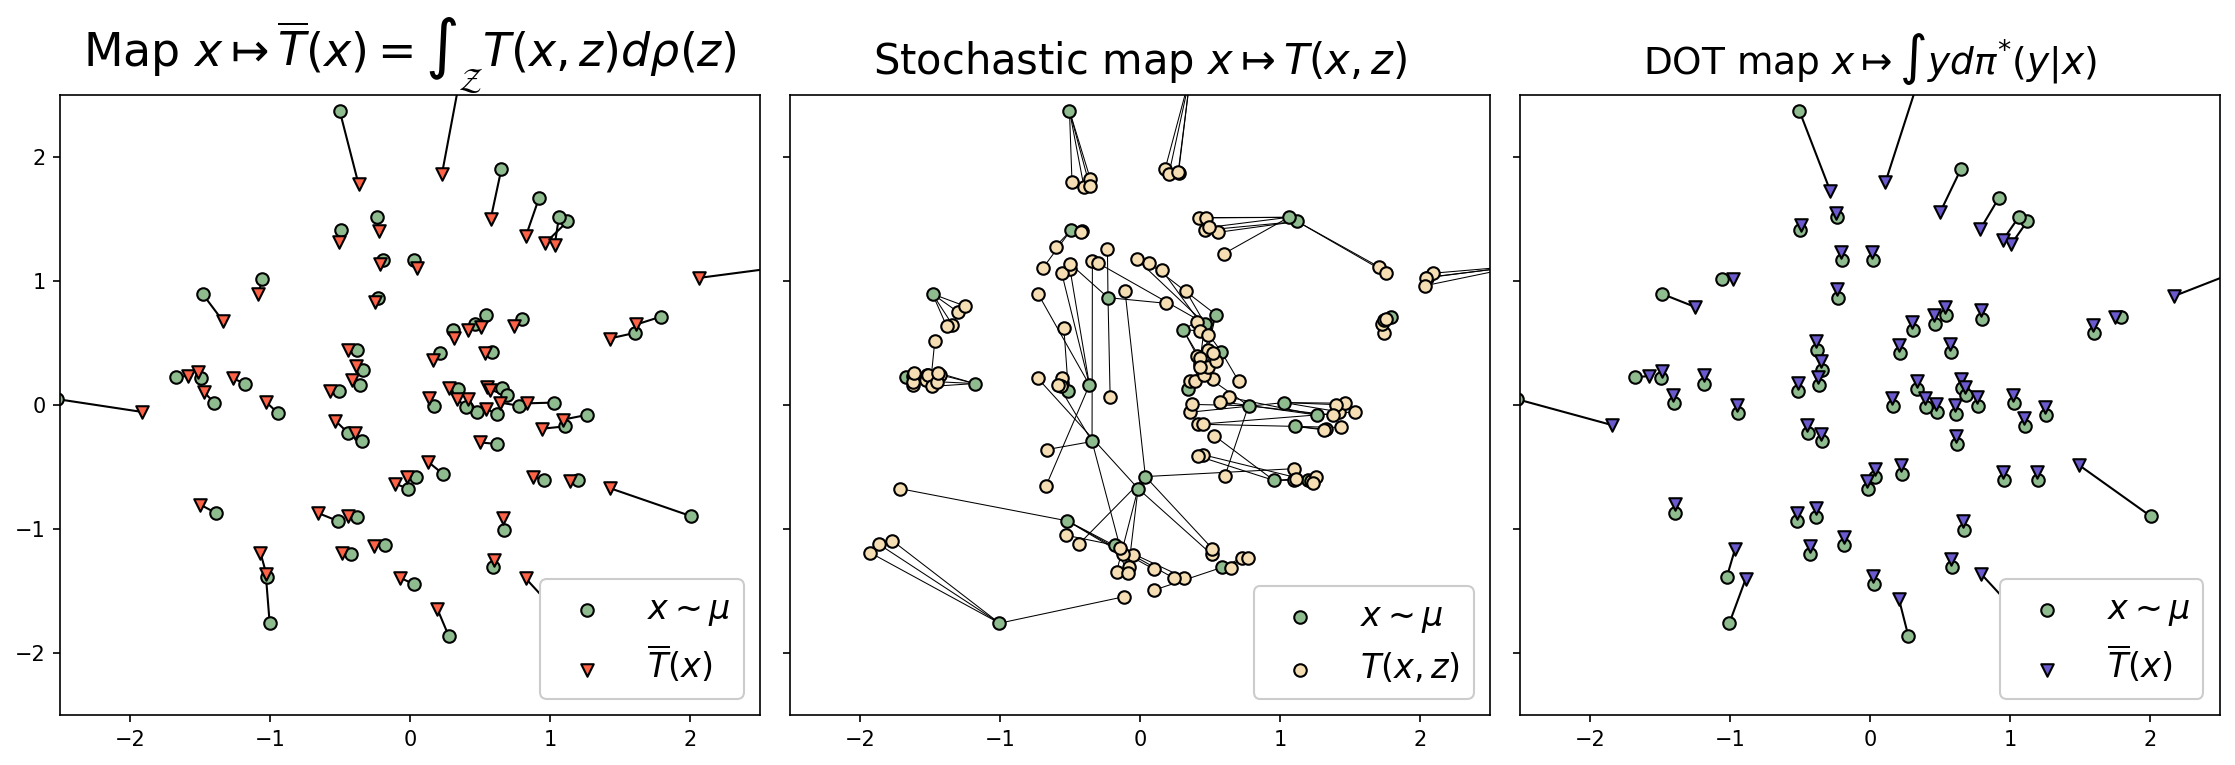
\includegraphics[width=0.9\textwidth]{figures/toy_2.png}
        \caption{Synthetic data experiment. Left: average of the learned transport for different points. Middle: learned transport for a batch of points. Right: optimal transport plan obtained with the POT library.}
        \label{fig:toy_2}
    \end{figure}
\end{frame}
\subsection{Large-scale dataset}
\begin{frame}{Large-scale dataset}
    \begin{itemize}
        \item CelebA dataset with 200k celebrity face images.
        \item CartoonSet with 100k avatar 2D generated images.
    \end{itemize}

    \begin{figure}[h!]
        \centering
        
\includegraphics[scale=.2]{figures/cartoonset-excerpt.png}
        \caption{Images samples from CartoonSet100K}
    \end{figure}
\end{frame}

\begin{frame}{Large-scale experiment: the parameters}
    \begin{itemize}
        \item Resnet to parametrise $f$.
        \item U-Net to parametrise the map $T$.
        \item image size: $128\times128$.
        \item Batch size: 128.
        \item Adam optimizer.
        \item $\text{lr} = 1\times10^{-4}$.
        \item $k_T = 10$.
    \end{itemize}
\end{frame}

\begin{frame}{Results: it works!}
    \begin{figure}[h!]
        \centering
        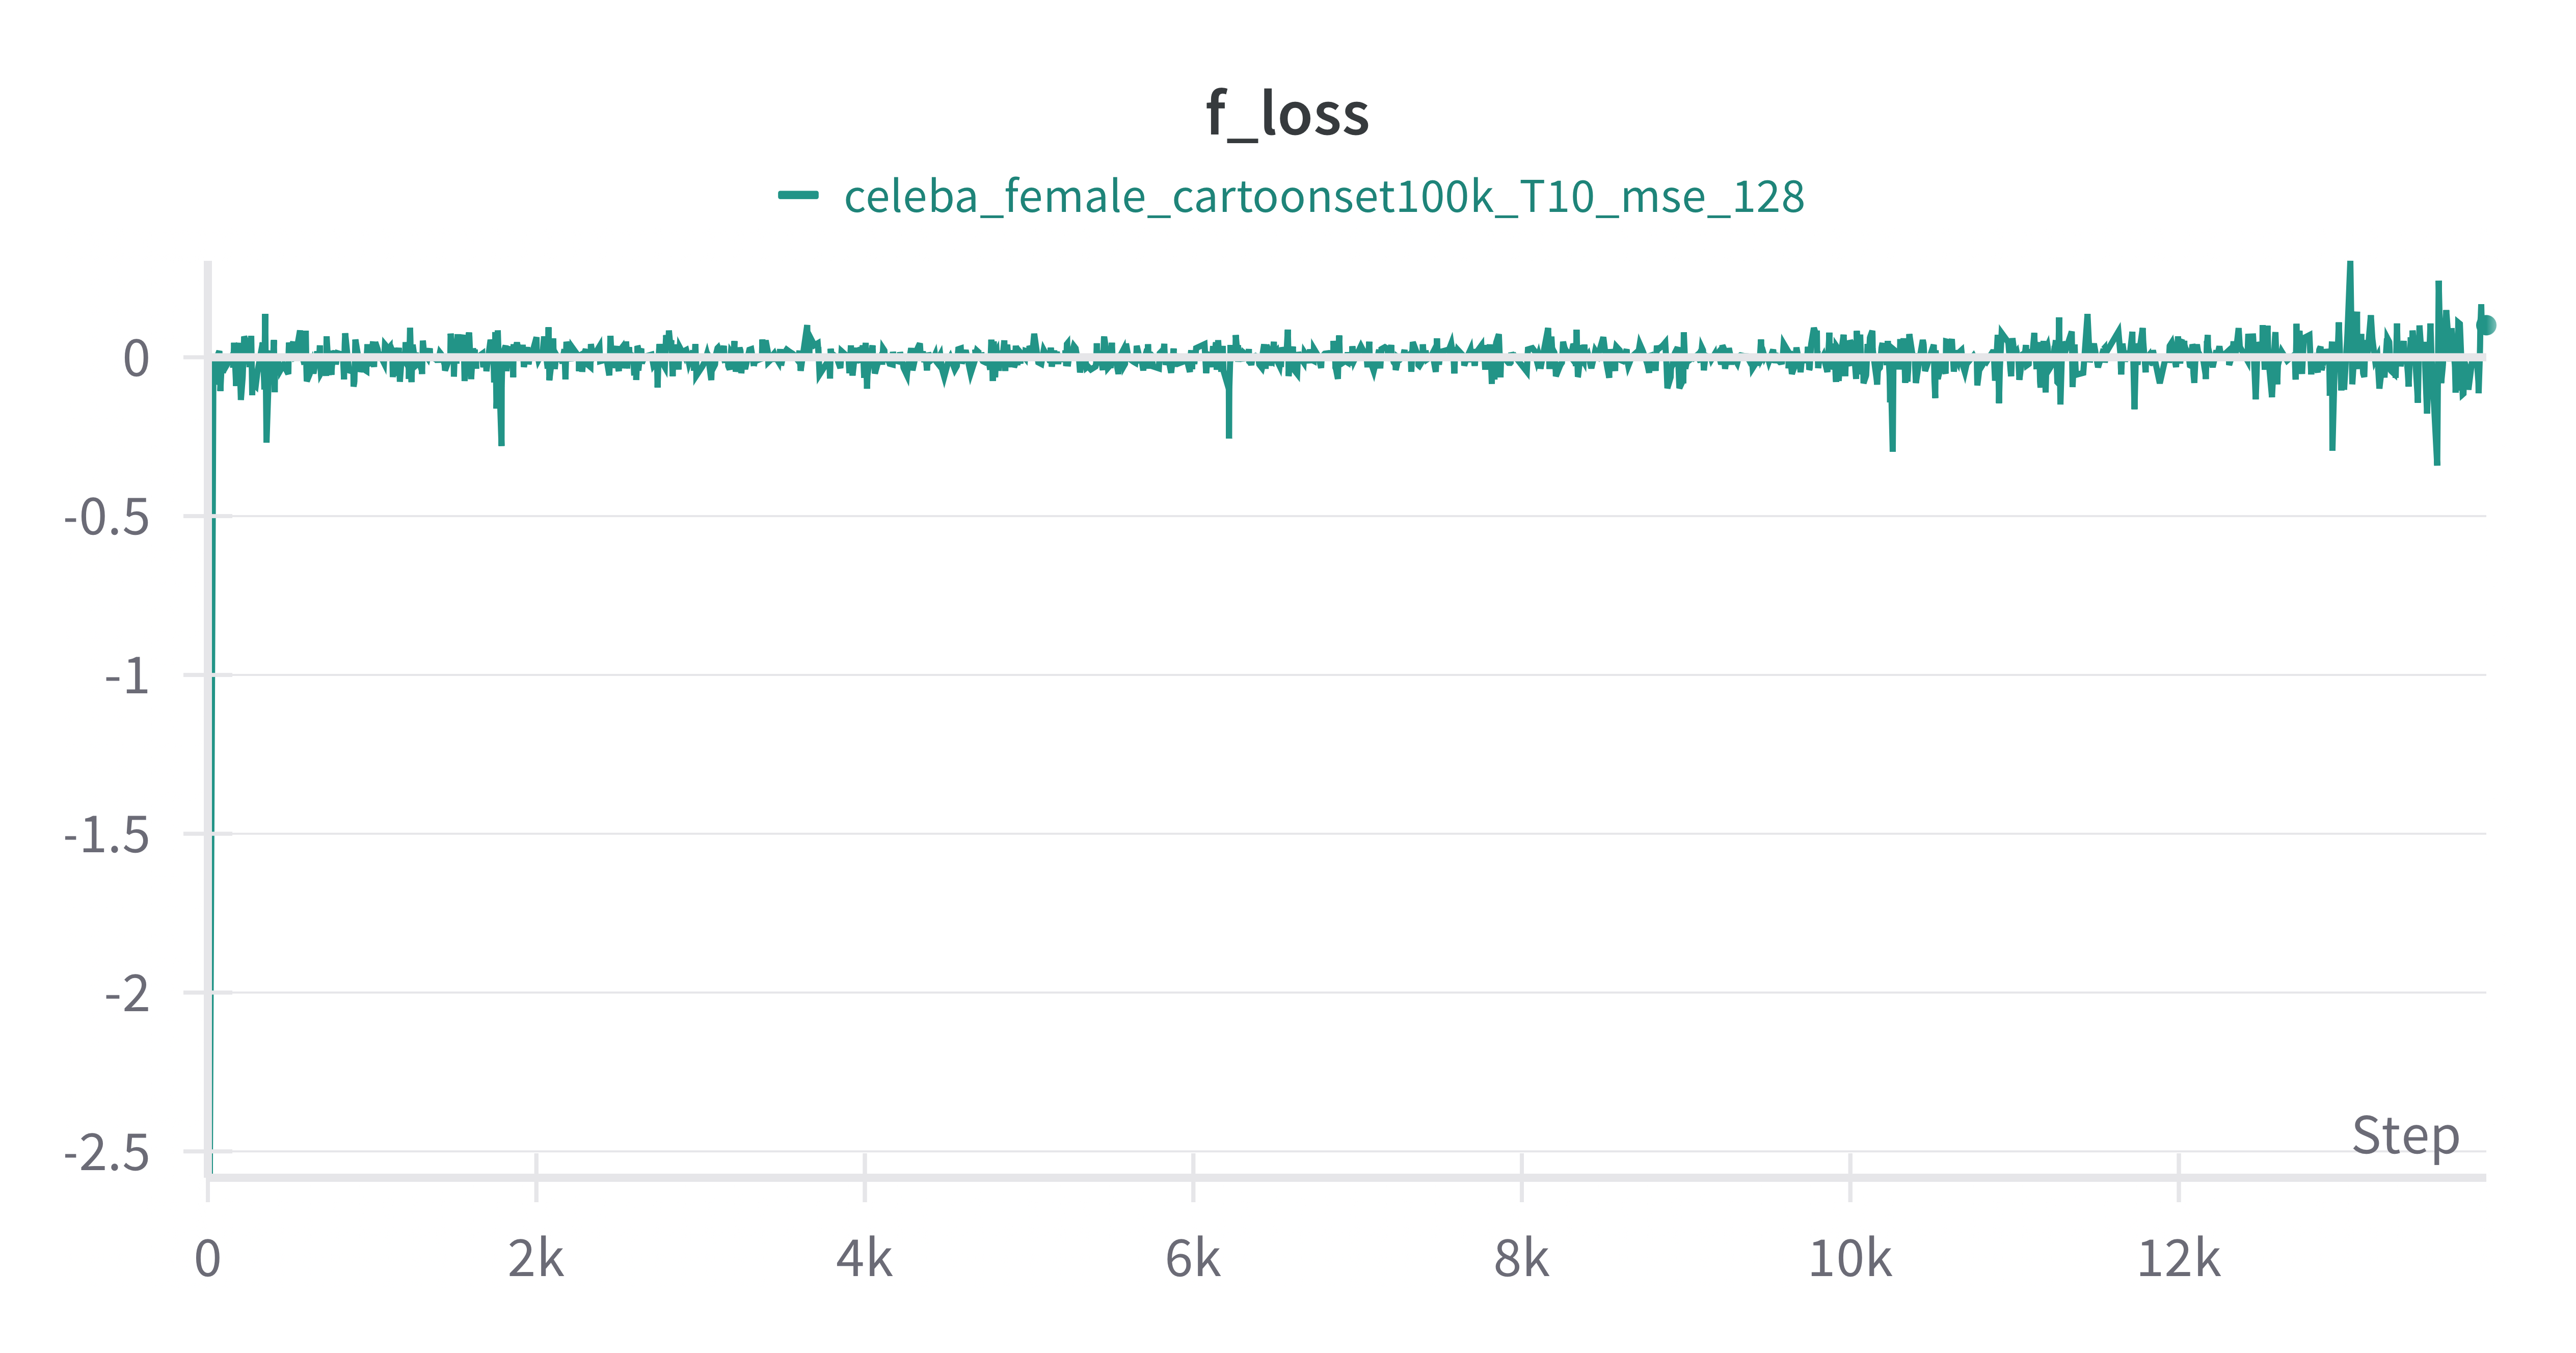
\includegraphics[scale=.05]{figures/loss_real_dataset.png}
        \caption{${\cal L}_f$ during training}
    \end{figure}
\end{frame}

\begin{frame}{Results: some generated avatars}
    \begin{figure}
        \centering
        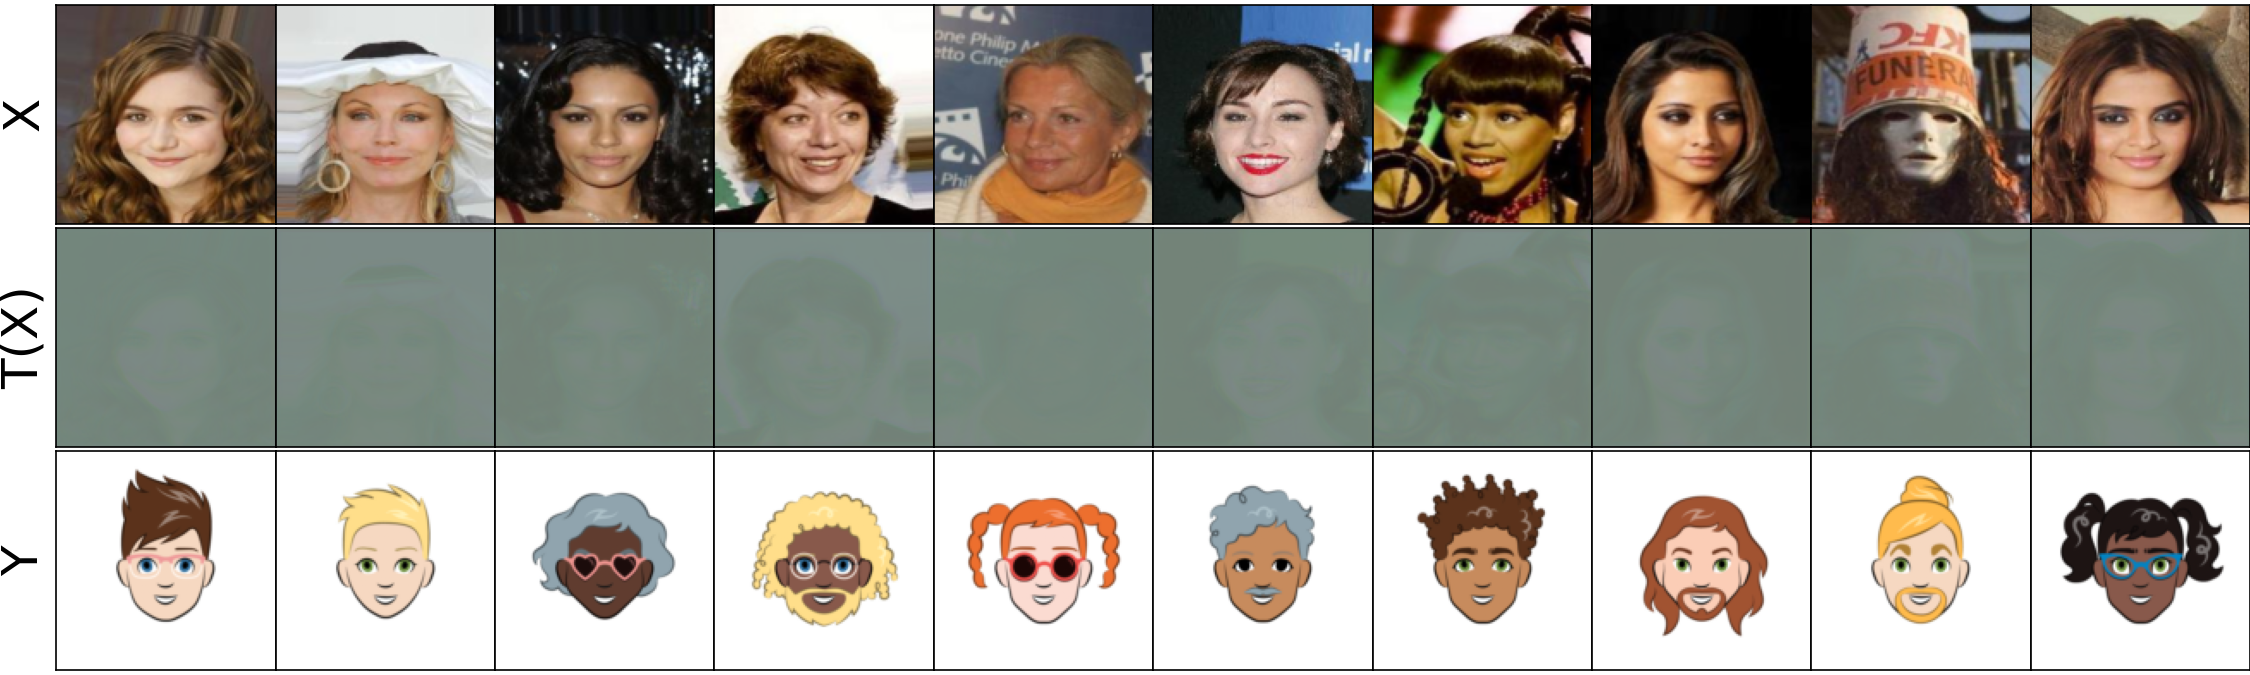
\includegraphics[scale=.1]{figures/media_images_Fixed Images_0_a56284c48d003ecfb6cd.png}
        \caption{Iteration 1}
        \label{fig:test_images_real_iter_1}
    \end{figure}
    \begin{figure}
        \centering
        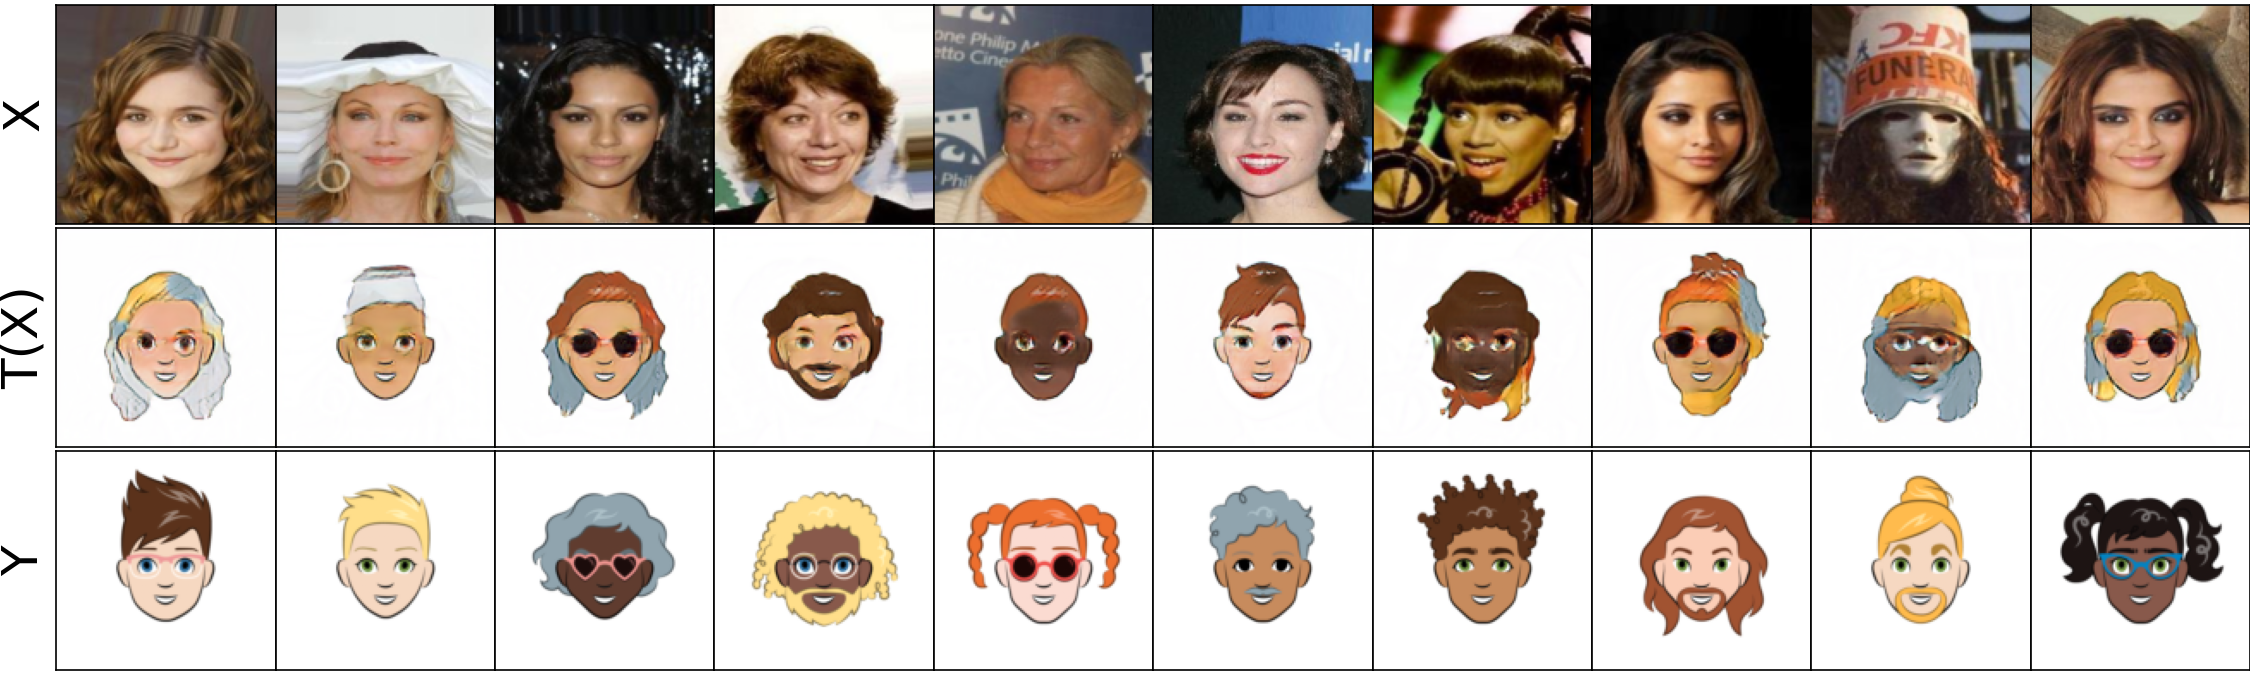
\includegraphics[scale=.1]{figures/media_images_Fixed Images_5000_0043c7527d827202e7ad.png}
        \caption{Iteration 5000}
        \label{fig:test_images_real_iter_med}
    \end{figure}
\end{frame}

\begin{frame}{Results: an issue}
    \begin{figure}
        \centering
        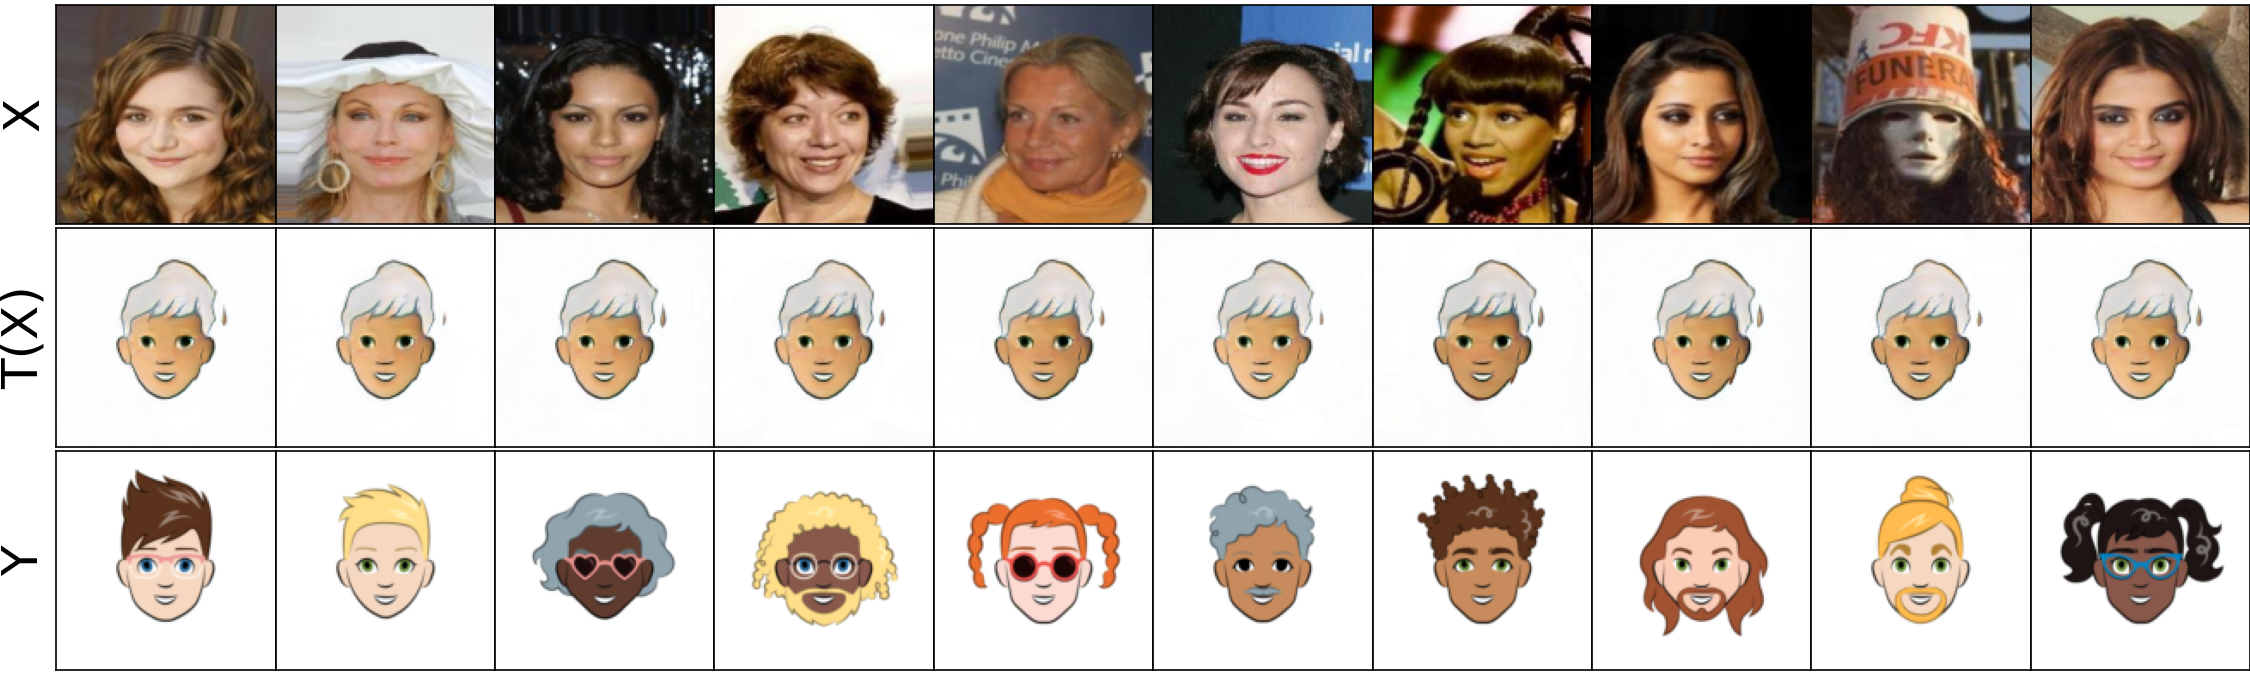
\includegraphics[scale=.1]{figures/media_images_Fixed Images_13800_653d5de40c4ba6a777ca.png}
        \caption{Iteration 13800}
        \label{fig:test_images_real_iter_last}
    \end{figure}
    \begin{itemize}
        \item Mode collapse!
    \end{itemize}
\end{frame}

\section{Conclusion}
\begin{frame}{Conclusion}
    \begin{itemize}
        \item An algorithm to learn optimal transport maps.
        \item New approach to incorporate OT in ML.
        \item With good results on large-scale datasets!
        \item Good perspectives for generative models.
    \end{itemize}
\end{frame}

\begin{frame}
    \bibliographystyle{amsalpha}
    \bibliography{bibliography}
\end{frame}

\end{document}